\documentclass[12pt,onecolumn]{article}
\usepackage{listings}
\usepackage{float}
\usepackage{mathtools}
\usepackage{hyperref}
\usepackage[russian]{babel}
\everymath{\displaystyle}
\usepackage{placeins}
\usepackage[table,xcdraw]{xcolor}
\usepackage{geometry}
\geometry{
  a4paper,
  top=25mm, 
  right=15mm, 
  bottom=25mm, 
  left=15mm
}

\begin{document}
\setcounter{tocdepth}{4}
\begin{center}
    Санкт-Петербургский Национальный Исследовательский\\ 
    Университет ИТМО\\
    Мегафакультет Компьютерных Технологий и Управления\\
    Факультет Программной Инженерии и Компьютерной Техники \\
    
\includegraphics[scale=0.3]{itm.jpg} % нужно закинуть картинку логтипа в папку с отчетом
\end{center}
\vspace{1cm}


\begin{center}
    \large \textbf{Вариант №311678876767.6}\\
    \textbf{Лабораторная работа №4}\\
    по дисциплине\\
    \textbf{Программирование}
\end{center}

\vspace{2cm}

\begin{flushright}
  Выполнил Студент  группы number\\
  \textbf{Student's name}\\
  Преподаватель: \\
  \textbf{Teacher's name}\\
\end{flushright}

\vspace{10cm}
\begin{center}
    г. Санкт-Петербург\\
    2021г.
\end{center}
\newpage
\tableofcontents
\newpage
\section{Текст задания}
\textbf{Программа должна удовлетворять следующим требованиям:}
\begin{itemize}
  \item В программе должны быть реализованы 2 собственных класса исключений (checked и unchecked), а также обработка исключений этих классов.
  \item В программу необходимо добавить использование локальных, анонимных и вложенных классов (static и non-static).
\end{itemize}
\textbf{Порядок выполнения работы:}
\begin{itemize}
  \item Доработать объектную модель приложения.
  \item Перерисовать диаграмму классов в соответствии с внесёнными в модель изменениями.
  \item Согласовать с преподавателем изменения, внесённые в модель.
  \item Модифицировать программу в соответствии с внесёнными в модель изменениями.
\end{itemize}
\textbf{Описание предметной области, по которой должна быть построена объектная модель:}\\
Нужно сказать, что Незнайка никогда не забывал о своём больном друге. Не проходило дня, чтоб он не забежал к нему хотя бы на минутку. Обычно это удавалось сделать во время послеобеденной прогулки. Всегда, когда Незнайка обедал с собаками, он не съедал свою порцию до конца, а припрятывал в карман то пирожок, то котлетку, то хлебца краюшку и относил всё это голодному Козлику.\\

В первый же день он обратился к госпоже Миноге с просьбой заплатить ему жалованье хотя бы за недельку вперёд, так как ему нужно помочь больному приятелю, который находился в дрянингской ночлежке. Госпожа Минога сказала, что теперь он живёт в богатом доме, в обществе приличных собак, и ему не пристало водить компанию с каким-то Козликом, который даже дома собственного не имеет, а обитает в какой-то ночлежке.\\

– Ни о каких таких Козликах я не желаю и слышать! – сказала она. Если же вы произнесёте при мне или при Мимишке с Роландом какоенибудь неприличное слово вроде «ночлежки», я вас уволю. Что же касается платы, то вы будете получать её раз в неделю, но только не вперёд, а по прошествии недели.\\
\newpage
\section{Диаграмма классов объектной модели.}
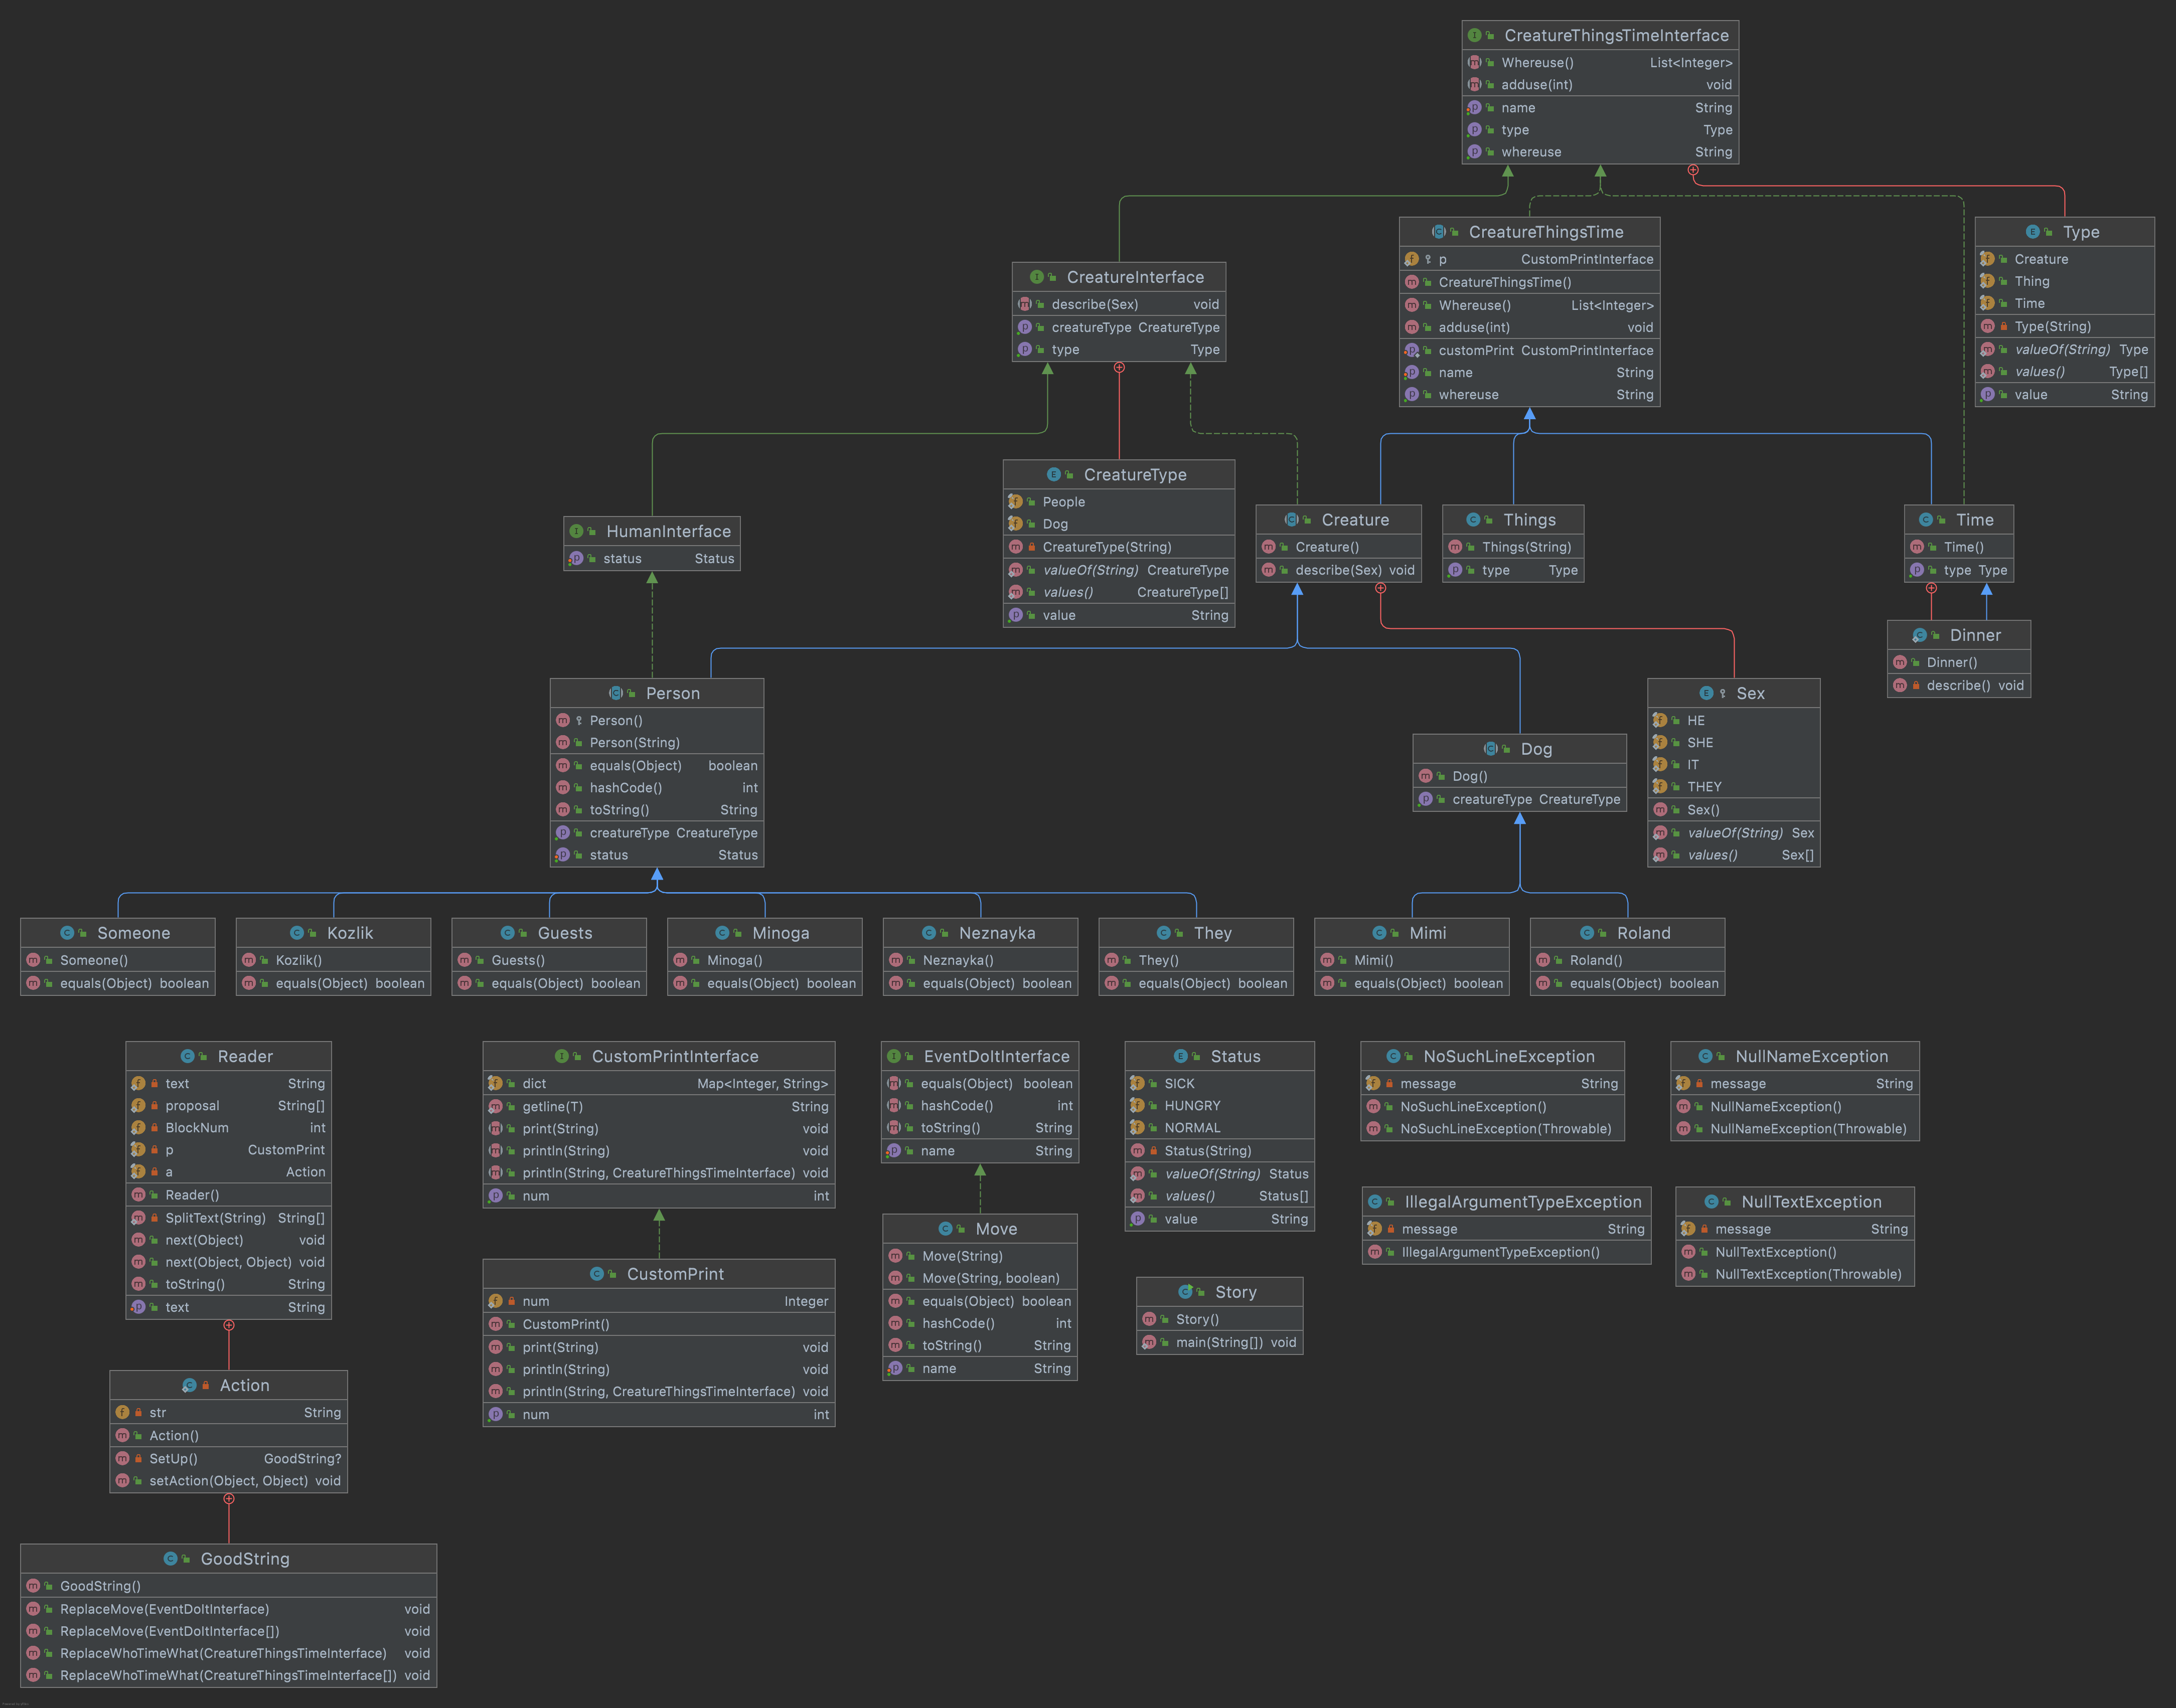
\includegraphics[scale=0.09]{UML.png}
\section{Исходный код программы}
\lstloadlanguages{Java}
\definecolor{mygray}{RGB}{120,120,120}
\lstset{extendedchars =/true,
breaklines=true,
basicstyle=\ttfamily\fontsize{9pt}{9pt}\selectfont,
commentstyle=\color{mygray},
keywordstyle=\color{blue},
}
Story.java
\lstinputlisting[language=Java,numbers=left]{../src/core/Story.java}
reader/Reader.java
\lstinputlisting[language=Java,numbers=left]{../src/core/reader/Reader.java}
print/CustomPrint.java
\lstinputlisting[language=Java,numbers=left]{../src/core/print/CustomPrint.java}
print/CustomPrintInterface.java
\lstinputlisting[language=Java,numbers=left]{../src/core/print/CustomPrintInterface.java}
exception\\
IllegalArgumentTypeException.java
\lstinputlisting[language=Java,numbers=left]{../src/core/exception/IllegalArgumentTypeException.java}
NoSuchLineException.java
\lstinputlisting[language=Java,numbers=left]{../src/core/exception/NoSuchLineException.java}
NullNameException.java
\lstinputlisting[language=Java,numbers=left]{../src/core/exception/NullNameException.java}
NullTextException.java
\lstinputlisting[language=Java,numbers=left]{../src/core/exception/NullTextException.java}
event\\
EventDoItInterface.java
\lstinputlisting[language=Java,numbers=left]{../src/core/event/EventDoItInterface.java}
Move.java
\lstinputlisting[language=Java,numbers=left]{../src/core/event/Move.java}
CreatureThingsTime\\
Creature.java
\lstinputlisting[language=Java,numbers=left]{../src/core/CreatureThingsTime/Creature.java}
CreatureInterface.java
\lstinputlisting[language=Java,numbers=left]{../src/core/CreatureThingsTime/CreatureInterface.java}
CreatureThingsTime.java
\lstinputlisting[language=Java,numbers=left]{../src/core/CreatureThingsTime/CreatureThingsTime.java}
CreatureThingsTimeInterface.java
\lstinputlisting[language=Java,numbers=left]{../src/core/CreatureThingsTime/CreatureThingsTimeInterface.java}
Status.java
\lstinputlisting[language=Java,numbers=left]{../src/core/CreatureThingsTime/Status.java}
Things.java
\lstinputlisting[language=Java,numbers=left]{../src/core/CreatureThingsTime/Things.java}
Time.java
\lstinputlisting[language=Java,numbers=left]{../src/core/CreatureThingsTime/Time.java}
CreatureThingsTime/people\\
Guests.java
\lstinputlisting[language=Java,numbers=left]{../src/core/CreatureThingsTime/people/Guests.java}
HumanInterface.java
\lstinputlisting[language=Java,numbers=left]{../src/core/CreatureThingsTime/people/HumanInterface.java}
Kozlik.java
\lstinputlisting[language=Java,numbers=left]{../src/core/CreatureThingsTime/people/Kozlik.java}
Minoga.java
\lstinputlisting[language=Java,numbers=left]{../src/core/CreatureThingsTime/people/Minoga.java}
Neznayka.java
\lstinputlisting[language=Java,numbers=left]{../src/core/CreatureThingsTime/people/Neznayka.java}
Person.java
\lstinputlisting[language=Java,numbers=left]{../src/core/CreatureThingsTime/people/Person.java}
Someone.java
\lstinputlisting[language=Java,numbers=left]{../src/core/CreatureThingsTime/people/Someone.java}
They.java
\lstinputlisting[language=Java,numbers=left]{../src/core/CreatureThingsTime/people/They.java}
CreatureThingsTime/dog\\
Dog.java
\lstinputlisting[language=Java,numbers=left]{../src/core/CreatureThingsTime/dog/Dog.java}
Mimi.java
\lstinputlisting[language=Java,numbers=left]{../src/core/CreatureThingsTime/dog/Mimi.java}
Roland.java
\lstinputlisting[language=Java,numbers=left]{../src/core/CreatureThingsTime/dog/Roland.java}
\section{Результат выполнения:}
\tiny{
\begin{verbatim}
  0. Время ужина
  1. Наконец приходила пора ужина,
  2. после которого время проводили по-разному.
  3. На сцене появилась Госпожа Минога
  4. Если у Госпожа Минога был званый вечер,
  5. На сцене появился Незнайка
  6. На сцене появилась Мими
  7. На сцене появился Роланд
  8. то Незнайка приводил Мими и Роланд в комнаты,
  9. На сцене появились гости
  10. На сцене появились собаками
  11. чтоб гости могли полюбоваться собаками.
  12. Если Госпожа Минога уходила в театр,
  13. то обязательно брала с собой и Мими,
  14. потому что в то время была мода таскать по театрам своих комнатных собачонок.
  15. На сцене появился кто
  16. Всех,
  17. кто являлся в театр или на концерт без собаки,
  18. считали неимущими бедняками и смеялись над ними.
  19. В такие вечера на попеченье Незнайка оставался один Роланд,
  20. На сцене появились они
  21. и они отправлялись вдвоём в спортивный собачий зал или плавательный бассейн,
  22. где  смотрели какое-нибудь собачье состязание,
  23. На сцене появился Козлик
  24. Статус персонажа Козлик изменён на болен
  25. или же отправлялись в дрянингский «Тупичок» и навещали больного Козлик.
  26. Нужно сказать,
  27. что Незнайка никогда не забывал о своём больном друге.
  28. не проходило дня,
  29. На сцене появился он
  30. чтоб он не забежал к нему хотя бы на минутку.
  31. Обычно это удавалось сделать во время послеобеденной прогулки.
  32. Всегда,
  33. когда Незнайка обедал с собаками,
  34. он не съедал свою порцию до конца,
  35. а припрятывал в карман то пирожок,
  36. то котлетку,
  37. Статус персонажа Козлик изменён на голоден
  38. то хлебца краюшку и относил всё это голодному Козлик.
  39. В первый же день Незнайка обратился к Госпожа Минога с просьбой заплатить ему жалованье хотя бы за недельку вперёд,
  40. так как ему нужно помочь больному приятелю,
  41. На сцене появился который
  42. который находился в дрянингской ночлежке.
  43. Госпожа Минога сказала,
  44. что теперь он живёт в богатом доме,
  45. в обществе приличных собак,
  46. и ему не пристало компанию с каким-то Козлик,
  47. который даже дома собственного не имеет,
  48. а обитает в какой-то ночлежке.
  49. На сцене появился я
  50. – Ни о каких таких Козлик я не желаю и слышать!
  51. На сцене появилась она
  52. – сказала она.
  53. На сцене появилась вы
  54. Если же вы произнесёте при мне или при Мими с Роланд какое-нибудь неприличное слово вроде «ночлежки»,
  55. я вас уволю.
  56. Что же касается платы,
  57. то вы будете получать её раз в неделю,
  58. но только не вперёд,
  59. а по прошествии недели.
  60. to be continued...
  Госпожа Минога встречается в строчках [3, 4, 12, 39, 43]
  Незнайка встречается в строчках [5, 8, 19, 27, 33, 39]
  Козлик встречается в строчках [23, 25, 38, 46, 50]
  Строчка 47: который даже дома собственного не имеет,
  Строчка 51: На сцене появилась она
  Строчка 57: то вы будете получать её раз в неделю,
  
\end{verbatim}
}
\section{Вывод}
\normalsize
В процессе выполнения этой лабораторной работы я познакомился с исключениями в java.
Научился использовать локальные, анонимные и вложенные классы.
\end{document}